%%%%%%%%%%%%%%%%%%%%%%%%%%%%%%%%%%%%%%%%%
% Beamer Presentation
% LaTeX Template
% Version 1.0 (10/11/12) 
%
% This template has been downloaded from:
% http://www.LaTeXTemplates.com
%
% License:
% CC BY-NC-SA 3.0 (http://creativecommons.org/licenses/by-nc-sa/3.0/)
%
%%%%%%%%%%%%%%%%%%%%%%%%%%%%%%%%%%%%%%%%%

%----------------------------------------------------------------------------------------
%	PACKAGES AND THEMES
%----------------------------------------------------------------------------------------

\documentclass{beamer}

\mode<presentation> {
%\mode<handouts> {
%\mode<article> {


% The Beamer class comes with a number of default slide themes
% which change the colors and layouts of slides. Below this is a list
% of all the themes, uncomment each in turn to see what they look like.


%\usetheme{default}
%\usetheme{AnnArbor}
%\usetheme{Antibes}
%\usetheme{Bergen}
%\usetheme{Berkeley}
%\usetheme{Berlin}
%\usetheme{Boadilla}
\usetheme{CambridgeUS}
%\usetheme{Copenhagen}
%\usetheme{Darmstadt}
%\usetheme{Dresden}
%\usetheme{Frankfurt}
%\usetheme{Goettingen}
%\usetheme{Hannover}
%\usetheme{Ilmenau}
%\usetheme{JuanLesPins}
%\usetheme{Luebeck}
%\usetheme{Madrid}
%\usetheme{Malmoe}
%\usetheme{Marburg}
%\usetheme{Montpellier}
%\usetheme{PaloAlto}
%\usetheme{Pittsburgh}
%\usetheme{Rochester}
%\usetheme{Singapore}
%\usetheme{Szeged}
%\usetheme{Warsaw}

% As well as themes, the Beamer class has a number of color themes
% for any slide theme. Uncomment each of these in turn to see how it
% changes the colors of your current slide theme.

%\usecolortheme{albatross}
\usecolortheme{beaver}
%\usecolortheme{beetle}
%\usecolortheme{crane}
%\usecolortheme{dolphin}
%\usecolortheme{dove}
%\usecolortheme{fly}
%\usecolortheme{lily}
%\usecolortheme{orchid}
%\usecolortheme{rose}
%\usecolortheme{seagull}
%\usecolortheme{seahorse}
%\usecolortheme{whale}
%\usecolortheme{wolverine}

%\setbeamertemplate{footline} % To remove the footer line in all slides uncomment this line
%\setbeamertemplate{footline}[page number] % To replace the footer line in all slides with a simple slide count uncomment this line

%\setbeamertemplate{navigation symbols}{} % To remove the navigation symbols from the bottom of all slides uncomment this line
}

\usepackage{graphicx} % Allows including images
\graphicspath{{../figures}}
\usepackage{booktabs} % Allows the use of \toprule, \midrule and \bottomrule in tables
\usepackage{amsmath, amssymb, amsthm, gensymb,mathrsfs}%,eufrak}
\usepackage{hyperref}
\usepackage{tabularx}
\usepackage{longtable}
\usepackage{makecell}
\usepackage{multicol}
\usepackage{physics}

\newcommand{\uvec}[1]{\textbf{#1}}

\newcounter{excounter}
%\renewcommand{\thefpcounter}{\thechapter.\arabic{fpcounter}}
%\renewcommand{\thefpcounter}{\thesection.\arabic{fpcounter}}
\renewcommand{\theexcounter}{\arabic{excounter}}

\newtheorem{teorema}{Teorema}[section]
\newtheorem{definicio}{Definició}[section]

\usepackage[lastexercise]{exercise}

\graphicspath{{../figures}}

%----------------------------------------------------------------------------------------
%	 TITLE PAGE
%----------------------------------------------------------------------------------------

\title[Classification]{Classification} % The short title appears at the bottom of every slide, the full title is only on the title page

\author{Jordi Villà i Freixa} % Your name
\institute[FCTE] % Your institution as it will appear on the bottom of every slide, may be shorthand to save space
{
Universitat de Vic - Universitat Central de Catalunya \\
Study Abroad\\ % Your institution for the title page
\medskip
\textit{jordi.villa@uvic.cat} % Your email address
}
%\date{\today} % Date, can be changed to a custom date
\date{course 2023-2024}
\logo{
\includegraphics[width=.1\textwidth]{FCTE}}
\begin{document}

\begin{frame}
\titlepage % Print the title page as the first slide
\end{frame}

\begin{frame}
\frametitle{Índex} % Table of contents slide, comment this block out to remove it
\tableofcontents % Throughout your presentation, if you choose to use \section{} and \subsection{} commands, these will automatically be printed on this slide as an overview of your presentation
\end{frame}

%----------------------------------------------------------------------------------------
%	PRESENTATION SLIDES
%----------------------------------------------------------------------------------------
\section{Introduction and scope}
\begin{frame}
  \frametitle{Preliminary note}
  The material in these slides is strongly based on \cite{kroese2020}. When other materials are used, they are cited accordingly.

  Mathematical notation follows as good as it can a \href{https://ctan.math.utah.edu/ctan/tex-archive/macros/latex/contrib/mlmath/mlmath.pdf}{good practices proposal} from the Beijing Academy of Artificial Intelligence.
  \end{frame}

%------------------------------------------------
\section{Introduction} % Sections can be created in order to organize your presentation into discrete blocks, all sections and subsections are automatically printed in the table of contents as an overview of the talk
%------------------------------------------------

%\subsection{Subsection Example} % A subsection can be created just before a set of slides with a common theme to further break down your presentation into chunks

\begin{frame}{What to expect?}
  In this session we will discuss:
  \begin{itemize}
    \item Classification methods
    \item Zero-one loss
    \item Bayes error rate
    \item Classification metrics
  \end{itemize}
\end{frame}

\section{Classification methods}


\begin{frame}{Regression is a supervised learning method}
Supervised methods in which a categorical response variable $Y$ takes one of the possible $c$ values which is to be predicted from a vector of $\uvec{X}$ explanatory variables, using a prediction function $g$.\\[10pt]

As $g$ classifies the input $\uvec{X}$ into one of the classes, we call $g$ a classification function or, simply, a {\em classifier}.\\[10pt]

As with any supervised learning technique, the goal is to minimize the expected loss or risk
\begin{equation}
  \mathscr{l}(g)=\mathbb{E}\mathrm{Loss}(Y,g(\uvec{X}))
  \label{eq:risk}
\end{equation}
for some loss function $\mathrm{Loss}(Y,g(\uvec{X}))$ that quantifies the impact of classifying a response $y$ with $\hat{y}=g(\uvec{x})$.
\end{frame}

\begin{frame}{Zero-one loss}
    The zero-noe or {\em indicator} loss function is the natural choice: $\mathrm{Loss}(y,\hat{y}):=\mathbb{I}\{y\neq\hat{y}\}$: this is: there is no unit loss for a correct classification and a unit loss for wrong one.\\[10pt]
    This leads to the fact that we aim at taking  $g(\uvec{x})$ to be equal to the class label $y$ for which $\mathbb{P}[Y=y|\uvec{X}=\uvec{x}]$ is maximal.\\[10pt]
    The error we generate in this process is linked to the so-called \href{https://www.projectrhea.org/rhea/index.php/Upper_Bounds_for_Bayes_Error}{Bayes error rate}.
\end{frame}

\begin{frame}{Pre-classifier}
  For a given training set $\tau$, a classifier is foten derived from a pre-classifier $g_{\tau}$, which is a prediction function (learner) that can take any real value, rather than only values in the set of class labels.
  \begin{figure}
  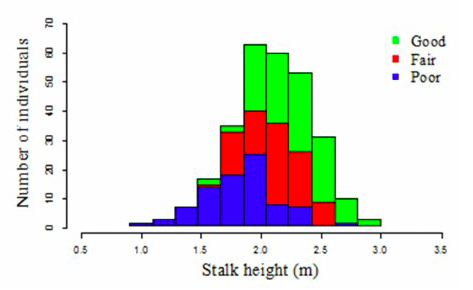
\includegraphics[width=0.7\linewidth]{continuous_classification}
  \caption{Adapted from \href{https://www.scielo.br/j/cbab/a/Z8D4PknkTQxQjfx8NF4CZwj/?lang=en}{here}}
\end{figure}
\end{frame}

\begin{frame}
  \begin{figure}
    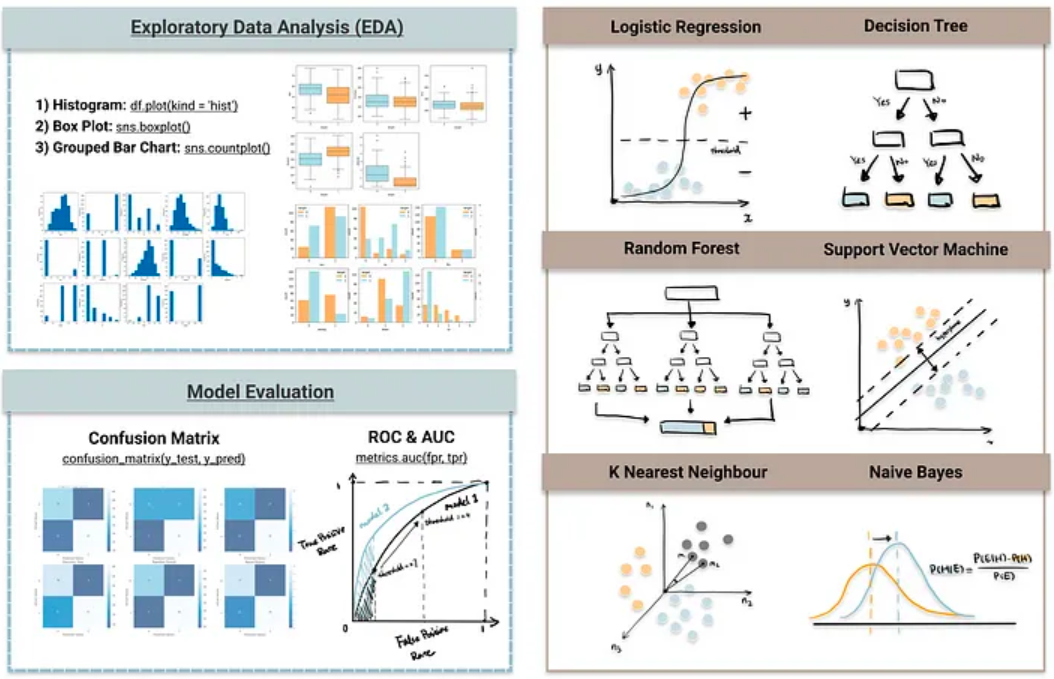
\includegraphics[width=0.8\linewidth]{classification}
    \caption{Check the \href{https://towardsdatascience.com/top-machine-learning-algorithms-for-classification-2197870ff501}{source} for a plain explanation of the different classification methods.}
  \end{figure}
  \end{frame}

\begin{frame}{Training and test sets. Loss ans confussion matrices}
  Theoretically, we should be measuring the risk in Eq. \ref{eq:risk} and minimizing such equation over some class of functions $\mathcal{G}$. However, as the training loss is often a poor estimate of the risk, this is usually estimated from the test set $\tau'$.
  \begin{description}
    \item[Loss matrix $\uvec{L}$]: for the indicator loss function, it contains 0 in the diagonal and 1 everywhere else.
    \item[Confusion matrix $\uvec{M}$]: counts the number of times that, for the training or test data, the actual (observed) class is $i$ whereas the predicted class is $j$. 
  \end{description}
  The training/test loss of the classifier in terms of $\uvec{L}$ and $\uvec{M}$ is 
  $\frac{1}{n}\sum_{i.j}[\uvec{L}\odot\uvec{M}]{ij}$
  In the case of the indicator loss, the missclassification error is $1-\tr(\uvec{M})/n$
\end{frame}

\begin{frame}{Confusion matrix}
 \begin{figure}
    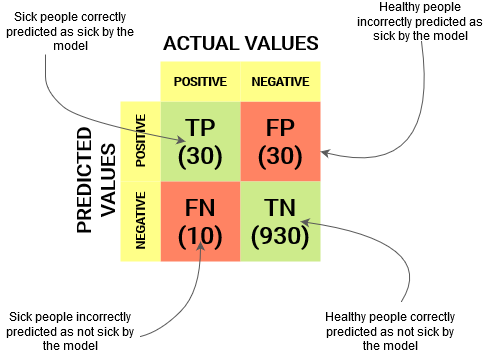
\includegraphics[width=0.7\linewidth]{Example-Confusion-matrix}
    \caption{Adapted from \href{https://www.analyticsvidhya.com/blog/2020/04/confusion-matrix-machine-learning/}{here}.}
 \end{figure}
\end{frame}

\begin{frame}{Missclassification error and accuracy}
  In the binary classification case ($c=2$), and using the indicator loss function, the missclassification error can be written as:
  \[
    \mathrm{error}_j = \frac{\mathrm{fp}_j+\mathrm{fn}_j}{n}  
  \]
  and the accuracy can be calculated by measuring the fraction of correctly classified objects:
  \[
    \mathrm{accuracy}_j = 1 -   \mathrm{error}_j = \frac{\mathrm{tp}_j+\mathrm{tn}_j}{n}
  \]
\end{frame}

\begin{frame}{Other classification metrics}
  We can do better than this in many situations:
  \begin{itemize}
    \item we can modify the loss matrix and make it different from the indicator
    \item we can modify the the way we measure the classification beyond the accuracy_
    \begin{itemize}
      \item precision: $\mathrm{precision}_j = \frac{\mathrm{tp}_j}{\mathrm{tp}_j+\mathrm{fp}_j}$
      \item recall or sensitivity: $\mathrm{recall}_j = \frac{\mathrm{tp}_j}{\mathrm{tp}_j+\mathrm{fn}_j}$
      \item specificity: $\mathrm{specificity}_j = \frac{\mathrm{tn}_j}{\mathrm{tp}_j+\mathrm{fp}_j}$
      \item $F_{\beta}$ score: $F_{\beta}=\frac{(\beta^2+1)\mathrm{tp}_j}{(\beta^2+1) \mathrm{tp}_j+\beta^2 \mathrm{fn}_j+\mathrm{fp}_j}$
    \end{itemize}
  \end{itemize}
\end{frame}

\section{Bibliography}
\bibliographystyle{unsrt}
\bibliography{DataSciencewithPython}
\end{document}